\documentclass{sigchi}

% Use this command to override the default ACM copyright statement (e.g. for preprints). 
% Consult the conference website for the camera-ready copyright statement.
\toappear{
	Submitted for review.
}

% Arabic page numbers for submission. 
% Remove this line to eliminate page numbers for the camera ready copy
\pagenumbering{arabic}

% Load basic packages
\usepackage{balance}  % to better equalize the last page
\usepackage{graphics} % for EPS, load graphicx instead
\usepackage{times}    % comment if you want LaTeX's default font
%\renewcommand{\ttdefault}{cmtt}
%\usepackage{fontspec}
%\setmainfont{Cardo}
\usepackage{url}      % llt: nicely formatted URLs
\usepackage{dblfloatfix}
\usepackage{caption}

% llt: Define a global style for URLs, rather that the default one
\makeatletter
\def\url@leostyle{%
  \@ifundefined{selectfont}{\def\UrlFont{\sf}}{\def\UrlFont{\small\bf\ttfamily}}}
\makeatother
\urlstyle{leo}

\newcommand{\msb}[1]{\textbf{\textcolor{cyan}{Michael: #1}}}
%\newcommand{\cir}{{context-independence }}


% To make various LaTeX processors do the right thing with page size.
\def\pprw{8.5in}
\def\pprh{11in}
\special{papersize=\pprw,\pprh}
\setlength{\paperwidth}{\pprw}
\setlength{\paperheight}{\pprh}
\setlength{\pdfpagewidth}{\pprw}
\setlength{\pdfpageheight}{\pprh}

% Make sure hyperref comes last of your loaded packages, 
% to give it a fighting chance of not being over-written, 
% since its job is to redefine many LaTeX commands.
\usepackage[pdftex]{hyperref}
\hypersetup{
pdftitle={SIGCHI Conference Proceedings Format},
pdfauthor={LaTeX},
pdfkeywords={SIGCHI, proceedings, archival format},
bookmarksnumbered,
pdfstartview={FitH},
colorlinks,
citecolor=black,
filecolor=black,
linkcolor=black,
urlcolor=black,
breaklinks=true,
}

\usepackage{array} % for defining a new column type
\usepackage{varwidth} %for the varwidth minipage environment

% create a shortcut to typeset table headings
\newcommand\tabhead[1]{\small\textbf{#1}}
\newcolumntype{A}{>{\begin{varwidth}{1cm}}l<{\end{varwidth}}}
\newcolumntype{B}{>{\begin{varwidth}{2cm}}l<{\end{varwidth}}}
\newcolumntype{C}{>{\begin{varwidth}{3cm}}l<{\end{varwidth}}}
\newcolumntype{D}{>{\begin{varwidth}{4cm}}l<{\end{varwidth}}}



% End of preamble. Here it comes the document.
\begin{document}

\title{Interactive formal reasoning for large online courses}

\numberofauthors{1}
\author{
  \alignauthor Ethan Fast, Colleen Lee, Alex Aiken, Daphne Koller, Michael Bernstein, Eric Smith\\
    \affaddr{Stanford University}\\
    \email{\{ethan.fast, clee0, aiken, koller, msb, eric\}@cs.stanford.edu}\\
}

\maketitle

\begin{figure*}[ht!]
\centering
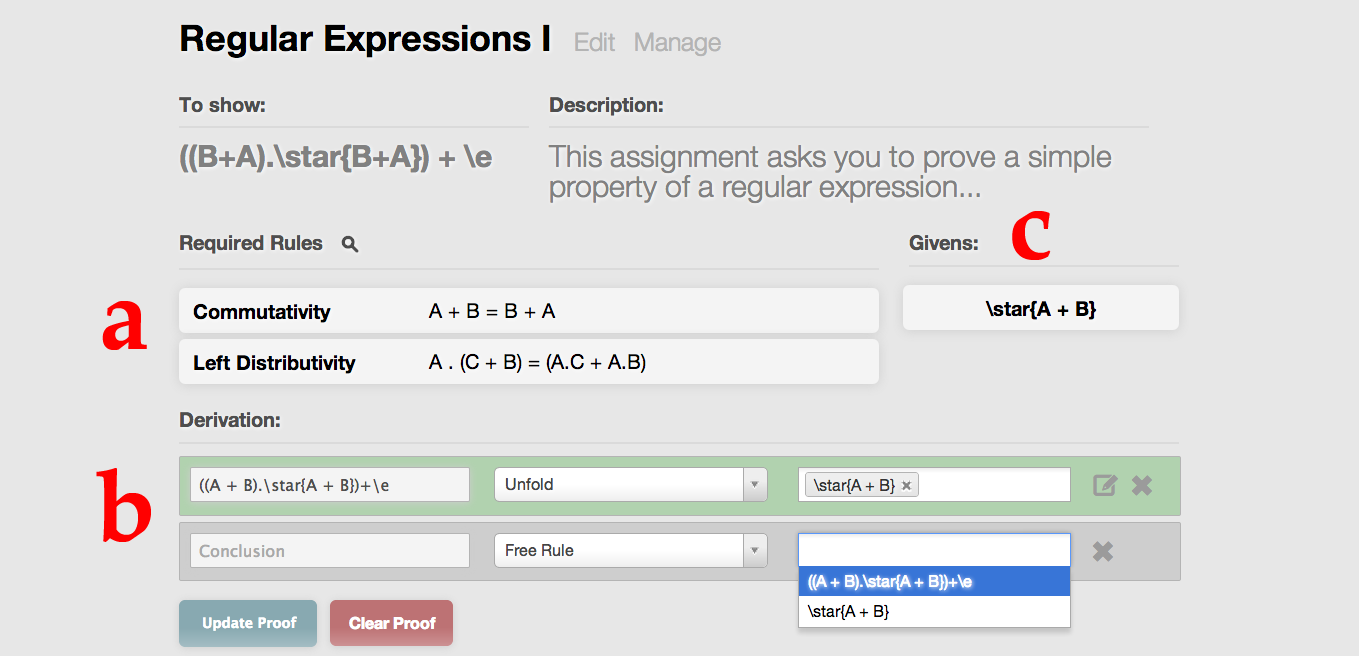
\includegraphics[width=1\textwidth]{splash3}
\caption{The DeduceIt interface: (a) set of available rules (b) interactive derivation component (c) set of given assumptions}
\label{fig:splash}
\end{figure*}

\begin{abstract}
Large online courses often assign problems that are gradable by simple checks such as multiple choice, but these checks are inappropriate for domains in which students may arrive at many different valid solutions. One such domain is \emph{derivations}: sequences of logical steps commonly used in assignments for technical, mathematical and scientific subjects. We present DeduceIt, a system for creating and grading derivation assignments across arbitrary formal domains with many valid solutions. DeduceIt supports assignments in any logical formalism, and it allows instructors to specify the level of abstraction at which each assignment may be completed --- students may elide steps which are didactically unimportant to a derivation. The system is scalable and accessible to many thousands of students on the web. DeduceIt benefits from the constraint of checking many thousands of user derivations: it introduces the idea of a \textit{proof cache}, a novel data structure which leverages a crowd of students to decrease the cost of checking derivations and providing real-time, constructive feedback. We evaluate DeduceIt with 990 students in an online compilers course, finding that students take advantage of its incremental feedback and that instructors benefit from its structured insights into confusing course topics.
\end{abstract}

\keywords{
	MOOC, theorem prover, formal logic, online education
}

\category{H.5.2}{Information Interfaces and Presentation}{Graphical user interfaces}

% See: \url{http://www.acm.org/about/class/1998/}
% \textcolor{red}{Mandatory}

\terms{
	Human Factors; Design 
}

% \url{http://www.sheridanprinting.com/sigchi/generalterms.htm}.
% \textcolor{red}{Optional section to be included in your final version.}


% Interactive assignments for large online courses 

% Interactive formal assignments in large online courses

 

\section{Introduction}
As online courses enroll thousands of students \cite{enroll}, course staff are unable to provide feedback on assignments and instead turn to automatic grading systems. Automatic grading works well for some assignments such as multiple choice quizzes, but it remains difficult to automatically evaluate assignments in complex domains where students may construct correct solutions in many different ways \cite{automated-scoring-design, automated-grading}. 

% Michael: that vs. which can be confusing. Easiest heuristic is whether you enclose it in commas. "I'm sure the chair, which is his favorite, will fall over." vs. "I'm sure that favorite chair will fall over." In this sentence, I don't think you need either of them.
This paper addresses the design of a system built to evaluate \textit{derivations}: sequences of logical steps where each step follows from some number of its predecessors. Technical, mathematical, or scientific subjects often assign such derivations in their traditional, offline problem sets. We are interested in a system that provides generality in two respects: assignments may be 1) defined in any formal domain, and 2) completed by students at specifiable levels of abstraction.

We adopt a broad view of assignment evaluation. While a simple grading system can tell a student whether an answer is correct (e.g., through multiple choice or string matching), it doesn't know enough about a student's reasoning to provide guidance in the event that an answer is wrong. We aim to provide \textit{constructive} suggestions which enhance learning \cite{personalized-feedback}.

Similarly, students tend to learn better when subject to \textit{real-time} feedback loops, for example help from human TAs in a traditional course setting \cite{personalized-feedback, derivation-scoring}. However, most existing grading systems constrain assignments to single-valued solutions and offer students limited feedback, typically unassociated with the intermediate steps of a solution \cite{coursera-doc}. For derivations this limitation is problematic; they are prone to a great deal of internal variation, and often have many right answers \cite{derivation-scoring}. 

%Interface design is also a concern for these systems. \textit{Oviatt et. al} suggest that as a system departs further from a traditional ``pen and paper" interface, a greater cognitive load is placed upon the student \cite{interface-learning-load}. This again suggests that systems which rely upon simplifications to an assignment's answer domain (e.g. multiple choice, or a single solution field) are not ideal for working through a derivation.

Finally, to be useful in a MOOC, a good system must also be \textit{scalable}, capable of handling a workload of many simultaneous students. Since we are concerned with a system designed to work with derivations, this constraint is particularly important; checking formal logic is an expensive computation \cite{bisearch}.

To address these limitations we present:
%(e.g. in our Compilers course we use it to assign problems in type checking, regular expressions, finite automata, and many other topics; its generality allows its use in most formal systems).
\begin{itemize}
\item The \textit{DeduceIt} system: A web-based framework which allows instructors to to specify a general class of derivation exercises, scales to a large workload of students, and enables students to complete assignments at varied levels of abstraction. DeduceIt provides students with constructive and real-time feedback.
\item The idea of a \textit{proof cache}: A novel data structure which records the history of every attempted derivation, reusing computations from previously derived steps. We show that this cache can increase system efficiency by 87\% and provide feedback in less than one second.
\item An \textit{empirical evaluation} of DeduceIt: a deployment of DeduceIt to several thousand students online for assignments in type checking, regular expressions, finite automata, and several other topics. We detail how: 1) students take advantage of DeduceIt's incremental feedback for exploration 2) instructors use DeduceIt to obtain structured insights into confusing course topics.
\end{itemize}

The rest of this paper is organized as follows: we begin with related work and a motivating example, then we present DeduceIt's interface and capabilities. Next, we describe the implementation of the system and provide an empirical evaluation, using data collected from students in an online class. We close with reflections, conclusions, and future work.

\section{Related Work}
At its core, DeduceIt is an interactive proof solving system. Many existing tools provide users with rich and automated feedback as a form of proof assistance \cite{coq,maude,isabelle, isabelle1,lisp-logic}, but these tools provide unconstrained interfaces which are generally unsuited to the MOOC audience. For instance, tools like \textit{coq} and \textit{isabelle} allow users to explore complex problem domains in a terminal-like environment, but these interfaces require knowledge of an underlying programming language which is not usually accessible to lay students or, depending on the course in question, even to a typical instructor. Thus, while these tools are useful and expressive---isabelle has been used to encode ideas as nuanced as Godel's Incompleteness Theorem---they require too much background knowledge for the general educational context.

Some prior work has looked specifically at applying automated theorem provers in an educational setting \cite{suppes, suppes-prover}. In fact, DeduceIt draws a great deal on the insights of researches like \textit{Suppes}, and the idea of using theorem provers to enable education has engendered much discussion among researchers \cite{automated-grading, automated-scoring-design}. However, even systems designed to address educational use have tended toward interfaces which require a significant amount of outside knowledge; they typically require unstructured interactions with a terminal-like environment. Moreover, no such system has been deployed at web scale to serve thousands of students.

Other work has addressed automatic feedback and grading systems with a more domain specific focus. Simple forms of automatic grading have been studied in both physical and online classrooms \cite{auto-grade}. These systems tend to restrict an assignment's answer domain with assumptions like multiple choice answers, concrete-valued answers (e.g., answers that match against a string or numerical value), or a set of test cases to evaluate a programming assignment. While restricting the answer domain can work well for certain subjects or applications, in general it does not grant an instructor sufficient means to evaluate more creative or complex assignments. Various exceptions exist here as well: for instance, automated grading and plagiarism detection systems have long evaluated student program code---where solutions may be unstructured and creative---in computer science departments \cite{grade-programs, moss}, and also commercially. However, we are concerned here with less domain-specific solution: a system which works across all kinds of derivations.

Finally, crowdsourcing research has enabled new forms of problem-solving and evaluation. For instance, peer consistency evaluation can be used to effectively judge the accuracy---and grade---of a student's answer, even in the absence of a ground truth \cite{peer-consistency}; crowd-based peer assessment has been successfully applied to grade student assignments \cite{peer-assessment, chinmay-srk}; and crowds have been used to detect and generate various canonical features of a language, like code snippets for use in an IDE. \cite{crowd-snippets}. While DeduceIt's proof cache draws inspiration from crowd research---the system leverages the results of one student to help another---humans are never directly involved in assignment evaluation. We hope to further involve the crowd in DeduceIt's computations as a subject of future work.

\section{Scenario}
DeduceIt provides students with feedback and support for any formal domain, and allows instructors to specify the level of abstraction at which a student may work though a derivation. In this section, we demonstrate these ideas through a scenario from a student's perspective. 

\textit{Regular Expressions I} is an assignment we use to introduce students to DeduceIt. Here, students must show that two regular expressions are equal: $(A+B)* \equiv ((B+A).(B+A)*)+\epsilon$. We assign the syntax $+$, $*$, $\epsilon$, and $.$ as union, Kleene closure, empty string, and concatenation. Students must derive the expression $((B+A).(B+A)*)+\epsilon$ starting from a set of givens, in this case the single expression $(A+B)*$, using several properties regular expressions.

\subsection{Constraints on the Derivation Interface}

\textit{DeduceIt limits the actions available to students on each step of the derivation}. Students may freely enter expressions into the conclusion box of a derivation, but the rules and givens input fields are constrained to lists of possibilities. This offers students a form of guidance.

Since our student has been given only $(A+B)*$ from which to start her derivation, she reasons that she must select this expression from the givens input field on the first step. From the rule field she must select a rule from the list of assignment rules, and in the conclusion field she must enter a newly derived expression. She selects the ``Unfold" rule and tries it on the full starting expression, mentally applying the rule to the given to arrive at $((A + B).(A + B)*)+\epsilon$. Entering this in the conclusion input field, she submits the step. 

The derivation returns with her step highlighted in green: it was successful. A new set of input fields lies below her previous entry, querying her for the next step.

\subsection{Working at Specifiable Levels of Abstraction}
Since our student's previous conclusion is nearly identical to the goal, she wants to use it for her next step. If she can transform its two sub-expressions $A+B$ to $B+A$, then she will have proven the goal and completed the assignment. She decides to apply Commutativity to each of the two $A+B$ sub-expressions, entering her result in the conclusion input box on the next line of the derivation. This new conclusion is identical to the goal expression: $((B+A).(B+A)*)+\epsilon$

She selects ``Commutativity" from the rule input field, selects $((B+A).(B+A)*)+\epsilon$ from the givens field, and submits the step. DeduceIt checks her derivation, infers through proof search that she means to apply Commutativity twice---on the two appropriate sub-expressions---and responds that her derivation is correct. She has completed this assignment.

Here our student \textit{interacts with DeduceIt at a relatively high level of abstraction}: she applies Commutativity twice, simultaneously, in a single derivation step. Under a different assignment setup she might be required to enter each application of Commutativity separately. DeduceIt allows instructors flexibility in defining these sort of behaviors. %\msb{While this example is clear, it's not exactly an impressive use of the feature. I'd rather see one that allows the student to completely ignore a step (e.g., Commutativity) since it's obvious.}

\subsection{Providing Constructive and Real-time Feedback}

In this example, our student knows right away whether the intermediate steps of her derivation are valid. This allows her to move from one step to another with confidence that her prior reasoning is correct. Had she made a mistake on the first derivation step, the system would have told her about it; she need not worry about proceeding down a derivation path based in faulty reasoning. Moreover, had she been running DeriveIt on her own computer, it would have taken roughly four seconds for each piece of feedback. However, because DeriveIt can utilize proof steps that other students computed previously, she receives feedback in roughly half a second.


% \subsection{Completing a Derivation}
% As she reads over the assignment, our student realizes she has only been given one expression from which to start her derivation: $(A+B)*$. She reasons this must go in the givens input field on the first step. (In fact, this is the only expression DeduceIt allows her to enter in that field). Now she has two input fields left. One asks for a rule; the other a conclusion. To come up with a conclusion, she must decide which rule to apply, and where to apply it. She supposes ``Unfold" looks promising and tries it on the full starting expression, mentally computing:
% $$((A + B).(A + B)*)+\epsilon$$
% This expression looks pretty close to her goal, so she enters it in the conclusion input field. After selecting ``Unfold" as her rule, she tells DeduceIt to update her derivation. There is a brief computation, then the derivation returns with her previous step highlighted in green: it was successful. A new step lies below her previous entry---this one is empty---querying her for the next line of the derivation.
% 
% Our student now considers her previous conclusion: since it is nearly identical to the goal, she wants to use it for her next step. If she can transform its two sub-expressions $A+B$ to $B+A$, then she will have proven the goal and completed the assignment. While she is pretty sure one property of regular expressions does allow for this kind of transformation, she can't remember what it is called. So she looks through the assignment rules and sees it: Commutativity. Regular expressions are commutative under union.

% Now she applies Commutativity to each of the two $A+B$ sub-expressions, then enters her result in the conclusion input box on the next line of the derivation. This conclusion is identical to the goal expression: 
% $$((B+A).(B+A)*)+\epsilon$$
% She selects ``Commutativity" from the rule input box, chooses the conclusion from her previous step $((B+A).(B+A)*)+\epsilon$ as her new given, and tells DeduceIt to  update her proof. DeduceIt checks her derivation, infers through proof search that she means to apply Commutativity twice---on the two appropriate sub-expressions---and responds that the derivation is correct: she has completed this assignment.
% 
% This example illustrates several notable aspects of DeduceIt. First, DeduceIt limits the actions available to our student on each step of the derivation. While she may freely enter expressions into the conclusion box of a derivation, the rules and givens fields are constrained, offering a form of guidance. 
% 
% Second, in her application of the Commutativity rule, our student interacts with DeduceIt at a relatively high level of abstraction; she is able to apply the rule twice, simultaneously, in a single derivation step. Using a different assignment setup, she might be required to enter each application of Commutativity separately. DeduceIt allows instructors flexibility in defining these sort of behaviors. 
% 
% Finally, DeduceIt provides feedback immediately: our student knows right away whether her deductions are valid. This allows her to move from one step to another with confidence that her prior reasoning is correct.

\section{DeduceIt}

We begin with background information about term rewriting systems, then we present an overview of DeduceIt's two primary interfaces: the instructor and student views.

\subsection{Background: Term Rewriting Systems}
%\msb{Shortening this. Please check I didn't change any meaning unintentionally.}
DeduceIt uses a term rewriting system to verify student derivations. Term rewriting systems consist of a set of expressions with nested sub-expressions, and relations which define transformations on those expressions; each transformation is called a rewrite rule \cite{rewriting-logic, isabelle}. Term rewrite rules have a left side, which must match a term for the rule to be applied, and a right side, which defines the new expression produced by the rule. Variables may appear in the rule (declared in the system with $\$$ notation) which binds to the term or its subexpressions. For example, in a language which supports integers, symbols, and the binary operators $+$, $-$, and $=$ (this happens to be a subset of the default DeduceIt language), one such rule might be: $(\$x+\$y=\$z) \rightarrow (\$x=\$z-\$y)$. The system can apply this rule to the expression $2+1=3$ to produce $2=3-1$.

While DeduceIt's derivation checker operates primarily as a term rewriting system, it differs from a standard system in several respects. First, rewrite rules which assume context independence (declared with $:=$ instead of $\rightarrow$) can be applied recursively upon term subexpressions; the entire term need not match the rule, but only a subexpression of that term. This makes DeduceIt more efficient at verifying certain common derivations. Second, DeduceIt supports call outs to custom functions \cite{dynamic-rules}. For instance, if DeduceIt is provided with a set of rules which govern basic arithmetic  and the expression $x=3-1$, it can derive $x=2$ by using the dynamic rule $\$x-\$y := eval(\$x-\$y)$.

%Fixme: talkabout conditional rules

\begin{figure}[tb]
\centering
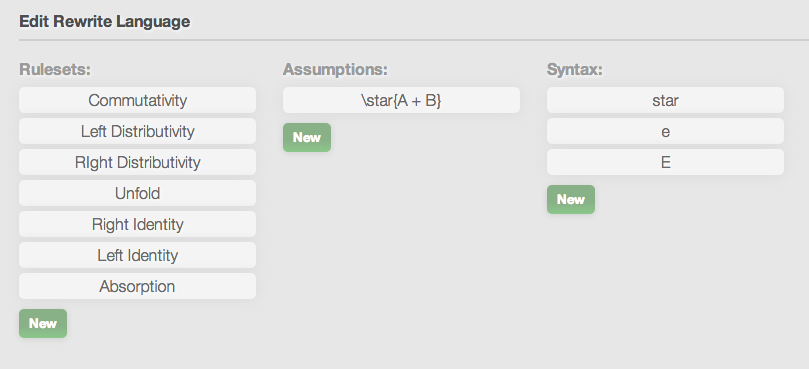
\includegraphics[width=1\columnwidth]{rewrite_language}
\caption{Instructors must specify a rewrite language for each assignment.}
\label{fig:rewrite_language}
\end{figure}

\begin{figure}[tb]
\centering
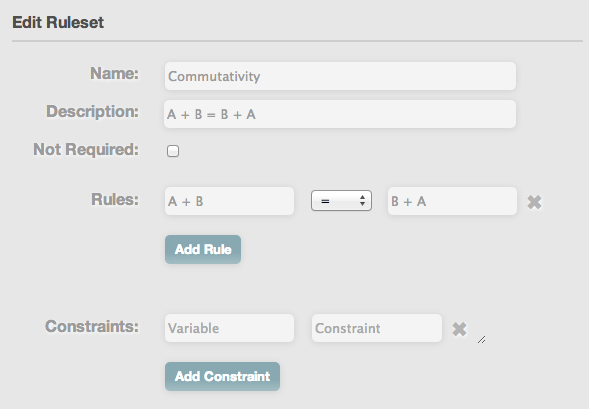
\includegraphics[width=1\columnwidth]{editruleset}
\caption{Editing a ruleset on the instructor interface.}
\label{fig:editruleset}
\end{figure}

\subsection{Assignment Creation Across Arbitrary Formalisms}

Instructors can use DeduceIt to define nearly any kind of formal assignment. To create an assignment, an instructor must specify four things: 
  \begin{enumerate}
  \item Rewrite language: Every assignment has a default rewrite language composed of variables, symbols, integers, and several common unary and binary operators. In many assignment domains this will be sufficient, but an instructor may optionally augment the language with extra syntax for functions and constants (Figure~\ref{fig:rewrite_language}). 
  \item Rulesets: Named sets of rewrite rules which a student may apply while working through an assignment's derivation. One ruleset corresponds to many underlying rewrite rules. This is necessary because an instructor may want to refer to several distinct rules by the same name (e.g., $1*X \rightarrow X$ and $X*1 \rightarrow X$ are two distinct rewrite rules describing the multiplicative identity.)
  \item The given expression(s): A set of expressions which serve as the starting point of a derivation.
  \item The goal expression: The desired result of a derivation.
  \end{enumerate}

A student works through an assignment by starting from the given expressions and applying valid transformations until she has reached the goal expression. %\msb{Note for later: to avoid the gender pronoun problem, I often give up some measure of grammatical correctness and use ``they'', or more correctly, pluralize ``users'' and then use ``they''.}

\subsubsection{Customizing an Assignment Language}

DeduceIt's default language is similar to that of an advanced calculator. It provides the unary operators $\char`\~$ and $-$, and the binary operators $.$, $\&$, $|$, $,$, $*$, $\backslash$, $+$, $-$, $=$, $\neq$, $\leq$, $\geq$, $<$, $>$, $=>$, $:=$, and $\rightarrow$, listed in order of precedence. DeduceIt also supports variables (only used when defining rewrite rules), symbols, and integers. For example, three legal expressions in the default rewrite language are: ``$\$p,(\$p=>\$q)\rightarrow{}\$q$'' ``$a.b.b.a$'', and ``$x+2=y$''.

Note that with three exceptions (the notation specific to rewrites: $:=$, $\rightarrow$, and $\$$) the operators used in expressions have no meaning without an accompanying set of rules; they simply determine the parsing of an expression.

Instructors may add two kinds of syntax to DeduceIt's standard rewrite language: constants and variable argument functions. This is convenient in many domains, where familiarly named functions and constants enhance the readability of an assignment. For these custom functions and constants DeduceIt adopts a notation inspired by LaTeX. Constants appear in the language as a symbol value preceded by a backslash, e.g $\backslash{}e$. Functions look much the same, except they have arguments which they accept in brackets, e.g., $\backslash{}sin\{x\}$.

\subsubsection{Defining an Assignment Domain with Rulesets}

Rulesets define the sets of valid transformations which a student may use in a derivation. Each ruleset has a name, a student-facing description, a set of rewrite rules, and an optional set of constraints (Figure~\ref{fig:editruleset}). The name and description of a ruleset are all a student sees when using DeduceIt, and these fields  make an assignment more accessible; students do not need to understand rewrite rules to use the system.

%\msb{Moved this to a more visible location. It gets a bit ahead of itself, but I think it's worth it to make sure the reader is still paying attention.} 
To allow students to elide less important proof steps, the instructor may choose whether a ruleset is \emph{required} or \emph{free}. Required rulesets must be named explicitly when a student uses them in a derivation. Free rulesets, however, may be elided. Behind the scenes, DeduceIt will attempt to fill in free steps automatically through proof search. This is useful when a student must use trivial transformations which are necessary to the derivation but unimportant to the assignment. For example, a student may want to collapse terms in a mathematical expression as part of some broader rule application. Consider a rewrite rule defining integration $\int{a^x} \rightarrow a^{x+1}/(x+1)$ and the given expression $\int{(a^2+0)}$ along with other rewrite rules governing basic algebra. A student might try to complete the integration immediately, deriving $a^3/3$, without providing the intermediate step $\$x+0 \rightarrow \$x$, which requires the addition property of zero. If an instructor marks the rewrite rule which governs the addition property of zero as free, DeduceIt will allow the student to skip this intermediate step, filling it in through proof search. %\msb{Again, this is clear because it's simple, but makes the thing seem kind of basic. I'd recommend a slightly more complicated example, perhaps with $\int{(a^2+2a^2)}$}.

DeriveIt separates rewrite rules into \emph{strict rewrite rules} and \emph{context independent rules}, which impacts whether the student must completely isolate the instance of the rule in order to apply it. To apply a strict rewrite rule, its left side must match exactly on an expression, wheres a content-independent rule may be applied to an expression or any of its subexpressions. Take as an example the expression $1+y*y=5$ and the strict rewrite rule $\$x*\$x \rightarrow \$x^2$; here the rewrite rule cannot be applied, since its left side doesn't match the entire expression. However, a similar rewrite rule which has been defined with an assumption of context independence, $\$x*\$x := \$x^2$, will match $y*y$ and produce the transformation $1+y^2=5$. For many assignments a single context independent rule can take the place of many strict rules. This eases the burden on an instructor and usually speeds up proof search; the more rules an assignment has, the slower search tends to be.

However, strict rewrite rules cannot be entirely replaced with context independent rules. Some transformations may be context dependent (e.g., lexing character values of a string). Moreover, strict rewrite rules allow instructors to simulate complex assignment domains which would otherwise lie outside the scope of a typical rewrite rule based system. For instance, we use strict rewrite rules to define a type checking assignment over a specific domain of input $\backslash{}type\{t\}\{expr\}$. Because we tailor such rules specifically to the context of this assignment, we do not need the power of full type analysis: rewrite rules are sufficient. %FIXME: Elaborate %This power at times seemed to surprise students. \msb{This description needs a more specific example. What power? What did it do?} Perhaps unaware of the system's intended generality, one student told us that the Compilers class ``has proven [DeduceIt] is as effective at teaching algorithms as it is at teaching proofs.''

%\msb{This paragraph seems less relevant. I recommend cutting or explaining more fully why this is important.} Constraints may be defined on the variable terms used in the ruleset. These constraints operate in a manner similar to conditional rewrite rules, but are somewhat less general; we use only containment---whether or not a variable contains certain other terms---as a condition on ruleset application.

% msb: probably not important enough for a heading \subsubsection{Sharing Rewrite Languages}
Some rewrite languages are common enough that it makes sense to share them among different assignments: for instance, many assignments might use the languages defined for basic algebraic manipulation, predicate logic, or the expansion of regular expressions. DeduceIt allows instructors to reuse a rewrite language across assignments.

%\msb{Many of these figures weren't referenced in the text. I recommend making sure each figure has at least one text anchor so that the reader knows when to look at it closely.}

\subsubsection{Assignment Analytics on the Proof Tree}
\begin{figure}[tb]
\centering
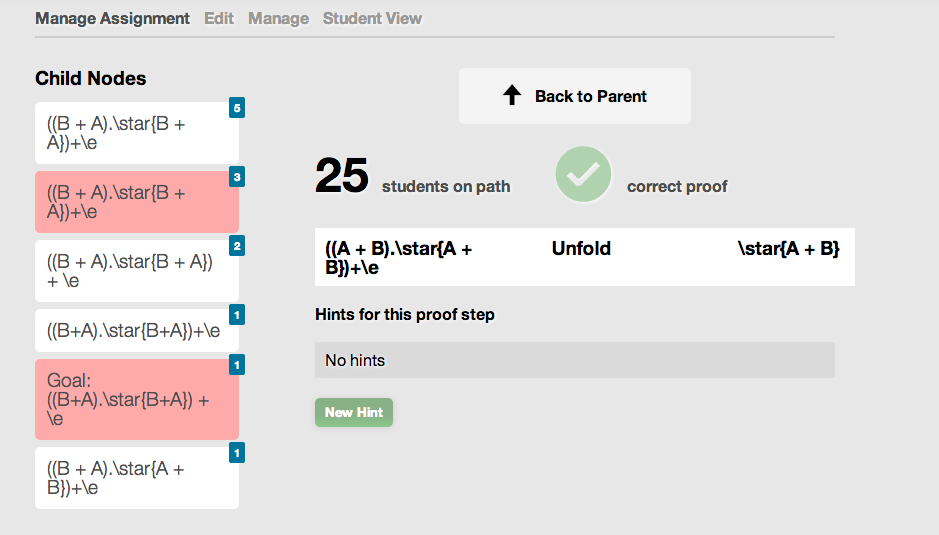
\includegraphics[width=1\columnwidth]{nodeannote}
\caption{Annotating a node on the proof tree.}
\label{fig:nodeannote}
\end{figure}

For each assignment, an instructor has real-time access to its \emph{proof tree} (Figure~\ref{fig:nodeannote}). The proof tree tracks the history of all derivations associated with the assignment. These derivations share a common root node, and each step in a derivation maps from a parent node to a child node via a ruleset transformation. Every node keeps track of derivation state information and a count of how many students have traversed it. An instructor may annotate any node in the tree with hints, and these will be visible to a student if she enters upon that path in her own derivation. An instructor may also use this tree to override the behavior of the underlying derivation checker, e.g., forcibly label a given derivation step valid. This can be useful for steps which make use of particularly long chains of free rules that aren't discovered and verified because of limitations in proof search. %TODO: Ask Michael, why confused about DAG?


\subsection{Interacting with a DeduceIt Derivation}

The student view (see Figure \ref{fig:splash}) broadly introduces the exercise at hand using the assignment's title, goal, and description. Below are the given expressions which a student uses to start the derivation and some number of rulesets divided into two types: required and free. Rulesets may be (and usually are) composed of many separate rewrite rules, but an assignment presents them as single, discrete entities; \textit{students need not be familiar with rewriting systems to use DeduceIt}. %In fact, the term `rewrite' cannot be found anywhere on the student view, and these rulesets are themselves labeled on the page simply as `rules'. This might create a leaky abstraction if rulesets are not carefully specified (i.e. the instructor description does not exactly match the behavior specified by the underlying rewrites), but most students are not familiar with rewrite rules, and we have discovered that a small sacrifice of precision in the rules positively impacts usability, as reported by several students.

Each assignment page contains an interactive derivation. Before a student has made progress in an assignment this derivation consists of only three empty input fields which are labeled: conclusion, rule, and givens. To more forward in a derivation, a student must derive a conclusion by applying the selected rule on the selected givens(s). 

\subsubsection{Constraints on a Derivation}

This derivation interface constrains students in several respects. First, students may select only expressions which they have already derived (or members of the set of starting givens) from the givens input field. Likewise, students may only select rules which are associated with the current assignment from the rules input field. These constraints eliminate the possibility of many simple mistakes, like typos, which we found surprisingly common in an earlier prototype of the system. The conclusion input field is unconstrained, however, and students can type into it any kind of expression they wish.

\subsubsection{Types of Derivation Feedback}

On each derivation step, DeduceIt responds with one of several kinds of feedback: if the derivation is so far valid, all its steps will turn green; if the system cannot parse the conclusion of some step in the derivation, that step will turn yellow; or if the system can parse but not prove the conclusion of some step in the derivation, that step will turn red. Each valid step preceding an invalid step will remain green, and if an invalid step has any hint annotations on the proof tree, a hint appears adjacent to that step. Hints take the form of a question mark, which expands into text on mouseover. Finally, if the conclusion of the latest step is equivalent to the goal expression, DeduceIt signals the assignment is finished with a checkmark and does not prompt for a new derivation step.

\subsection{Extensions to the Derivation Interface}

Based on our experiences with DeduceIt, we have developed several other forms of derivation feedback which we have not yet deployed for an online class.

\subsubsection{Surfacing the Proof Path}

DeduceIt maintains aggregate data about every derivation, so the system knows when students are proceeding down well-traveled paths in a derivation, or down correct but---so far---more lengthy paths, or down paths which have not yet led to the goal. One version of DeduceIt surfaces this information with a status indicator, a colored circle of green, yellow, or orange at the top of the derivation, indicating whether students are on a common path, an uncommon but successful path, or an as yet unsuccessful path. 

From anecdotal feedback, it seems students find this indicator helpful, and DeduceIt could provide students even finer grain information: the exact number of other successful or unsuccessful students who have worked to the current state of their derivation; or detection of the exact step in their derivation where they left the well-traveled path. It is also possible to further process the Proof Tree. By collapsing some nodes which are syntactically different but semantically equivalent (e.g., the expressions $(1+2)+3$ and $1+(2+3)$) we could construct a more meaningful notion of a derivation path. %\msb{Random thought: the representation mapping problem returns, just like in the code patterns project.}

\subsubsection{Providing Automatic Hints}

DeduceIt allows instructors to set up hints for any derivation step by annotating an assignment's proof tree. However, we built another version of DeduceIt that constructs these hints automatically using proof search. In this second implementation, DeduceIt holds the rule and assumption fields constant and searches for alternative valid conclusions. 

For instance, suppose that students enter $x=3+1$, \textit{Balance Equation}, and $x+1=3$ in the fields for conclusion, rule, and assumptions. This is an incorrect step, so DeduceIt will highlight it in red. And in the standard version of DeduceIt, if an instructor has not annotated this step on the proof tree, this is all the system will do. Students will only know the step is wrong. However, the hint-generating DeduceIt is able to give students more specific feedback, e.g., ``Balance Equation can be applied, but your conclusion is incorrect." Here proof search finds a viable alternative conclusion, $x=3-1$, so DeduceIt knows it is possible to apply the selected rule upon the selected given.

Other hint-generating systems might hold constant different parts of the derivation (e.g., searching for rules and assumptions to match a given conclusion). It is important that the system provide useful hints without giving away too much information: a tricky balance to achieve in an automated system. Hint generation is the subject of ongoing work.

\section{Implementation and Proof Cache}


DeduceIt is a system formed of three distinct components: a frontend interface, a backend theorem prover, and a database. The frontend manages all user interactions (for both students and instructors) as described in the previous section, the backend theorem prover exposes an online API which the frontend calls---when necessary---to check student derivations, and the database stores all the data associated with users and assignments, including the various proof trees which together constitute the proof cache. %\msb{So it's technically not a cache, e.g., stored in memcached? I bet it could be much faster.}

We built these components using several technologies and cloud providers. The frontend is a Ruby on Rails web application deployed on Heroku, the backend is a Haskell application also deployed on Heroku, and the database is a MongoDB installation running on MongoHQ. Each of these components can be scaled to serve arbitrary numbers of students.

\subsection{The Theorem Prover}

To verify student derivations, DeduceIt applies proof search over a term rewriting system. Its system differs from a standard rewriting system in that it supports rulesets (i.e., named groups of rewrite rules), context independent rules, dynamic evaluation for some term expressions, and conditions on the application of certain rewrites, as discussed earlier.

DeduceIt's theorem prover also includes a parser which the system constructs dynamically on each theorem prover call. This allows instructors to define custom assignment syntax. DeduceIt uses the parser to deconstruct the arguments of a theorem prover call into expression terms of the rewrite language before it passes these terms to the prover.

\subsubsection{The Theorem Prover API}

The DeduceIt prover is wrapped in a web server which can be queried via an API over the following arguments: \textit{rulesets}, \textit{assumptions}, \textit{syntax}, and \textit{conclusion}. To every query the prover will respond with either ``proven", ``unproven'', or ``syntax error.'' The frontend uses this API to assess the validity of each step in a derivation.

These arguments function much as their names suggest. The \textit{syntax} argument defines any new syntax on the default rewrite language. The rest of the parameters are used for proof search: DeduceIt tries to prove the provided \textit{conclusion} expression using the set of rewrite rules defined in \textit{rulesets} on the starting expressions in \textit{assumptions} (that is, assuming all these parameters parse). 

Although in the previous section we mentioned a student can select only one ruleset for each step of a derivation, it is usually necessary to pass the backend prover more than one ruleset; the prover requires not only the ruleset selected on the given step, but also any other rulesets which are declared ``free." Free rulesets are always allowed for any step of the derivation; in general they tend to be common or trivial transformations, orthogonal to the didactic goals of an assignment. 

\subsubsection{Proof Search}

Proof search applies rewrite rules iteratively upon a group of expressions to generate new expressions. In general, a search may be considered either \textit{forward}, starting from the known expressions and working toward the desired expressions, or \textit{backward}, starting from the desired expressions and working toward the known expressions with an inverted set of rules. DeduceIt supports both kinds of search. 

For example, suppose we give DeduceIt the assumption $a$, the rewrite rule $a \rightarrow a.a$, and the conclusion $a.a.a$. The system may conduct a forward search: start from $a$ and apply the rule twice, first producing $a.a$ and then $a.a.a$. Or it may search backward: construct a new rule $a.a \rightarrow a$ (the inverse of the old rule) and start from $a.a.a$, and then apply this new rule twice to produce $a.a$ and then $a$. Either method leads the system to declare the step valid.

In practice, DeduceIt conducts one round of forward search and one round of backward search; the two rounds of search then meet in the middle, i.e., they check for terms generated in common. We introduce backward search to ensure DeduceIt will correctly check rewrite languages which allow the introduction of new symbols, e.g., predicate logic and the rule $\$a \rightarrow \$a \vee \$b$ (note here that $\$b$ is a variable in the rewrite rule which binds to \textit{any expression}, so forward search cannot enumerate every possible value of $\$b$). Moreover, the meet-in-the-middle approach tends to be more effective than two rounds of only forward or backward search \cite{bisearch}.

We find the system is limited to two rounds of search under reasonable time constraints, with an upper bound of 4 seconds for students interacting with a web application. At each iteration of search DeduceIt applies the set of available rewrite rules---defined by the collection of rulesets---non-deterministically and exhaustively. Notably, this delay falls into the third classification of Nielsen's work on response times, beneath the ten-second limit for keeping a user focused on his or her dialog with the system \cite{neilsen}. While the theorem prover could be made more efficient, the next section will demonstrate that in many cases this is unneccessary.

\subsection{The Proof Cache}

The proof cache is a data structure DeduceIt uses to track all responses the frontend application receives from the prover. This cache is composed of many proof trees, one for each assignment, and together these proof trees track the aggregate history of every attempted derivation (as we discussed in Section 3). Proof trees are a useful tool for managing assignments---through them an instructor can annotate derivation steps and override the default behavior of the prover---but they can also, by acting as a cache, dramatically improve the overall performance of the system. 

DeduceIt's bottleneck is in its prover; proof search is by far the most computationally expensive aspect of the system. A proof cache can limit the outbound queries to the prover and so, intuitively, increase the performance of the system. 

To check a new derivation step using the proof cache, DeduceIt queries the proof tree associated with that derivation's assignment: if the new step already exists in the tree, then the system doesn't need to query the prover; it simply returns the stored result. %\msb{Why not use memcached with a concatenation of the given + ruleset as the key, and conclusion as the result? Avoids needing to bring the entire tree into memory.} Ethan: we hash the step information for faster tree lookups (the tree isn't in memory, either), but yeah, it could be a lot faster.

Besides the benefits of providing an infrastructure for hints and a summary of how well students are doing in an assignment, the proof cache has a very significant performance benefit for two reasons:
\begin{enumerate}
  \item Most students complete derivations with steps that other students have used previously or steps that will be used by future students.
  \item It is more efficient to reuse the intermediate results of one student's derivation to check the validity of another student's derivation than to check every derivation step with the prover. \label{hyp:2}
\end{enumerate}  
An average prover call takes $810ms$, whereas a typical cache lookup takes only $23ms$ seconds. Notably, this is an improvement which moves DeduceIt up a level on Nielsen's scale of responsiveness, under one second, to the level at which a user's flow of thought is uninterrupted \cite{neilsen}. We evaluate the performance impact of the proof cache more fully in the next section.

\section{Evaluation}

To evaluate DeduceIt we deployed it in the winter 2013 offering of Coursera's \textit{Compilers} class, which assigned each student several DeduceIt problems in every week of the course. Out of the 7625 students who enrolled, 990 of them completed at least one DeduceIt assignment. %Overall system latency was $1817ms$ on average.

In this section we provide evidence for two claims:

\begin{enumerate}
  \item \textit{DeduceIt successfully guides students through derivations}. We show through data analysis and anecdotal feedback that students engage with DeduceIt to solve problems.
  \item \textit{DeduceIt can provide instructors with insights that translate into future course improvements}. Here we provide examples from our experience with the Compilers course. 
\end{enumerate}
  
We run several analyses over ten DeduceIt assignments, measuring the distribution of students' time spent on assignments and derivation steps, the success rate of students, the average number of student errors, and the performance impact of the DeduceIt's proof cache.

\begin{figure}[!h]
\centering
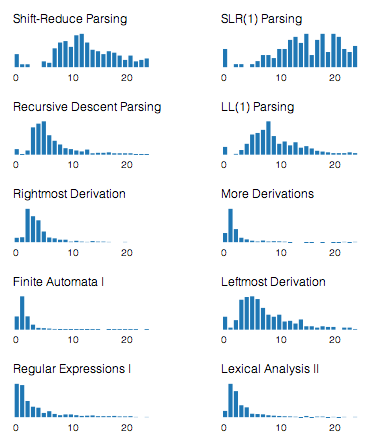
\includegraphics[width=1\columnwidth]{hist_short}
\caption{We construct normalized histograms to show the student time distributions for each assignment. The x-axis measures time in minutes.}
\label{fig:distributions}
\end{figure}

\begin{table*}[!ht]\footnotesize
  \renewcommand{\arraystretch}{1.5}
  \begin{tabular}{|p{3.4cm}|p{4.4cm}|p{.7cm}|p{.7cm}|p{.7cm}|p{.7cm}|p{.8cm}|p{.7cm}||p{.7cm}|p{.7cm}|}
    \hline
    \tabhead{Assignment Name} & \tabhead{Description} & \tabhead{Min} & \tabhead{Total} & \tabhead{Rules} & \tabhead{Cache} & \tabhead{Success} & \tabhead{Valid} & \tabhead{SX} & \tabhead{SM} \\
    \hline
    Regular Expressions I & \scriptsize{Prove two regexes are equivalent} & 2 & 185 & 7 & 3412 & 96\% & 55\% & 11\% & 34\% \\
    \hline
    Lexical Analysis II & \scriptsize{Show the sequence of moves of a lexer} & 6 & 119 & 4 & 5963 & 97\% & 63\% & 6\% & 30\% \\
    \hline
    Finite Automata I & \scriptsize{Show that an automaton accepts a string} & 5 & 53 & 10 & 4589 & 98\% & 73\% & 3\% & 23\% \\
    \hline
    Leftmost Derivation & \scriptsize{Perform a leftmost derivation} & 10 & 97 & 3 & 10857 & 95\% & 56\% & 6\% & 38\% \\
    \hline
    Rightmost Derivation & \scriptsize{Perform a rightmost derivation} & 10 & 78 & 3 & 10857 & 98\% & 81\%  & 1\% & 17\% \\
    \hline
    More Derivations & \scriptsize{Parse a sequence of roman numerals} & 6 & 61 & 9 & 9042 & 99\% & 81\% & 1\% & 18\% \\
    \hline
    Recursive Descent Parsing & \scriptsize{Show each state of a recursive descent parse } & 13 & 155 & 4 & 9465 & 96\% & 69\% & 1\% & 29\% \\
    \hline
    LL(1) Parsing & \scriptsize{Derive string using parse table} & 13 & 69 & 11 & 4750 & 99\% & 83\% & 1\% & 15\% \\
    \hline
    Shift-Reduce Parsing & \scriptsize{Show a shift-reduce parse of a string} & 20 & 151 & 8 & 6894 & 94\% & 85\% & 2\% & 12\% \\
    \hline
    SLR(1) Parsing & \scriptsize{Parse string using SLR(1) action table} & 15 & 99 & 33 & 4815 & 93\% & 60\% & 2\% & 36\% \\
    \hline
  \end{tabular}
  \caption{\textit{Min} is the shortest observed derivation path. \textit{Total} is the observed number of unique derivations paths. \textit{Rules} is the number of rules in the assignment. \textit{Cache} is the size of the proof cache, e.g., the observed number of unique steps. \textit{Success} is the success rate among students who attempted the assignment. \textit{Valid} is the percentage of derivation steps which are valid. \textit{SX} and \textit{SM} are the percentages of observed syntax and semantic errors, respectively. (Note: Leftmost and Rightmost Derivation share the same subset of the proof cache.)}
  \label{tab:table1}
\end{table*}

\subsection{Assignment Time Distributions}

First, we analyze the amount of time students spent on each assignment. Our results are displayed in Figure \ref{fig:distributions}. These time distributions are approximately normal with right skew and centered upon a fixed time value which tracks loosely with an assignment's difficulty. For example, in the \textit{Rightmost Derivation} assignment students are clustered around $4$ minutes, and in the \textit{Shift-Reduce Parsing} assignment they are clustered around $10$ minutes; the \textit{Rightmost Derivation} assignment is generally considered easier by students than the \textit{Shift-Reduce Parsing} assignment. This relation holds true among the remainder of the assignments. In general, we are heartened by the speed at which most students completed even the harder derivations. In offline assignments, instructors had to guess at difficulty with formal reasoning assignments or ask students, who may have faulty recall. %Fixme: flatten histograms a bit

\subsection{Rule Time Distributions}

We also observe the time distribution which governs rule application across assignments. Supposing some rules are easier or more natural to apply than others, we can use DeduceIt to find rules associated with longer elapsed time between steps, revealing what parts of the course material are more likely to confuse students. On average, it takes students 163 seconds to apply a rule in a derivation; around 3 minutes elapses between one derivation step and the next. 

We find that ``Nonterm Y input end'' is the rule associated with the longest elapsed time (1482s). This rule comes from \textit{LL(1) Parsing} and represents an operation on a lookup table. Most students using ``Nonterm Y input end'' have entered a valid but misleading conclusion on the previous derivation step, which is an ideal candidate for hint annotation on the assignment proof tree (e.g., a hint which suggests, ``While this step is correct, it doesn't lead to the solution.''). %Fixme: double check this stuff

For a second use-case of this data, we examine the assignment \textit{Regular Expressions I}. Here, the rules ``Left Identity'' and ``Right Identity'' are used by students most quickly, at about 100 seconds between applications. The ``Unfold'' rule is the most slowly used, at approximately 400 seconds in its application. This suggests Unfold may be the most challenging property of regular expressions for students to understand. 

More generally, these analytics grant the instructors fine-grained insight into students' understanding, even on complex assignments. Instructors might use such information to better focus the emphasis of their lectures.

\subsection{Student Success Rates}

Next, we examine the success rates of students across assignments. These results are displayed in table \ref{tab:table1}. Success rates are uniformly high, ranging from $93\%$ to $99\%$, and these rates track reported assignment difficulty in a manner consistent with time distributions. %\msb{Might be out of scope, but you could run a linear correlation on success rates vs. time spent, or even better, a multiple regression using success rate and time spent to predict self-rated difficulty. That could be quite useful.}

High success rates do not necessarily suggest that students are \textit{learning} from these assignments, but we have received feedback that supports this idea. Several students told us that they found DeduceIt's derivation constraints (e.g., a list of available rules and givens, and step-by-step validation) useful for understanding the domain of a problem. One student mentioned, ``Being able to step through the parsing actions and `be' the parser and know immediately when I made a mistake was incredibly helpful in coming to truly understand how the different parsing styles work.'' However, these constraints beget certain tradeoffs: DeduceIt trades flexibility in assignment notation for ease of verification, and other students told us that assignment syntax got in the way, that DeduceIt ``is difficult to use since you have to learn the syntax of each problem before actually applying what you know.'' An analysis of learning is outside the scope of this paper, but we see promise in such student feedback.

In general, high success rates show that students understand how to use DeduceIt and are engaging with assignments.

\subsection{Student Error Rates}

We next compute the rate of student mistakes across derivations, where an error is a conclusion which doesn't follow from the givens. Error rates among derivation steps for all the DeduceIt assignments are substantial---on average 29.4\%, or approximately one error for every three correct steps---despite the high overall success rates reported in Table~\ref{tab:table1}. We expect this result: students will always get some things wrong, and learning rarely takes place without error, whether indeliberate or in the form of exploratory, epistemic action \cite{citeulike}. Ideally, we might distinguish between two classes of error: errors which stem from a misunderstanding of course material, and errors which stem from misunderstandings (or exploratory actions) associated with the DeduceIt interface. %\msb{Recommend tying this to Kirsh and Maglio, Pragmatic vs. Epistemic action, to point out that students might be using the interactive system to explore options as a means of externalizing cognition.}

To approximate the impact of these two classes of error, we divide student mistakes into two categories: syntax errors, and semantic errors (SX and SM, Table~\ref{tab:table1}). Syntax errors arise from entering an expression which DeduceIt cannot parse, whereas semantic errors arise from parseable derivation steps which cannot be proven. While semantic errors are certain to contain faulty logic, this is not obviously true for syntax errors: a student might have intended to write a correct step and simply failed to use the system properly. We use the rates of student syntax errors as a proxy for measuring rates of student confusion with the DeduceIt system.

Across all assignments syntax errors are low, never exceeding $11\%$. Notably, the highest rate of syntax errors occurred in the first class assignment, \textit{Regular Expressions I}, despite the fact that students generally considered this assignment the easiest. The syntax error rates of subsequent assignments never exceeded $6\%$, although these later assignments were much more difficult. In fact, in the last 6 assignments, the average syntax error rate was only 1.3\%. This is likely a result of students learning to use the system. Low overall rates among syntax errors suggest that DeduceIt is not confusing students to the detriment of assignment completion and correctness.

\begin{figure}[!h]
\centering
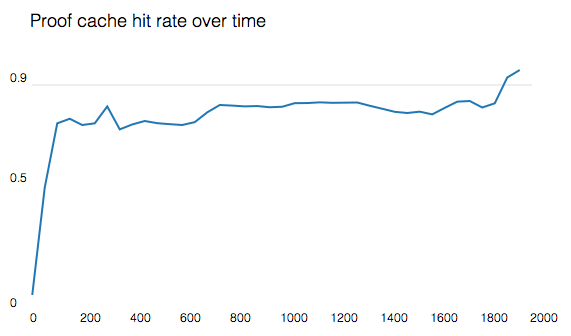
\includegraphics[width=1\columnwidth]{cache}
\caption{The x-axis measures the total number of derivation steps entered into the system. The y-axis measures the cache hit rate as a percentage.}
\label{fig:proofcache}
\end{figure}

\subsection{Performance Impact of the Cache}
First, we test a hypothesis which provides the general intuition behind the proof cache: \textit{most derivations contain steps that other students have previously used or will use in the future}. We counted the number of unique derivation steps entered into the class assignments. Of 50,099 total steps, only 5,407 (10\%) of them are unique. Since 90\% of derivation steps are reused, the data supports our first hypothesis.

Next, we examine our second hypothesis: \textit{it is more efficient to reuse the intermediate results of one student's derivation to check the validity of another student's derivation than to check every derivation step with the prover}. To test this hypothesis, we measured the overall proof cache hit rate. In Figure \ref{fig:proofcache}, we show the cache hit rate plotted against time. By the 1900th student interaction, the cache has reached a hit rate of $90\%$. Since the average theorem prover call takes $810ms$ and the average cache lookup takes $23ms$, we can compute an average time of $810ms*0.10+23ms*.90=101.7ms$. This represents a cost savings of 87\% and qualitatively improves usability: running the cache allows DeduceIt to move up one level on Nielsen's hierarchy of responsiveness \cite{neilsen}. %Fixme: calculate proper prover query

% High cache hit rates suggest that students tend to follow similar paths through their derivations. In table \ref{tab:table2} we show the number of unique assignment derivations compared against the overall cache hit rate for each assignment. [Fixme: acutally do this.]

% \subsection{System Performance}
% 
% In the final experiment, we measure the relation between system latency and load. Since a MOOC will typically enroll thousands of students, it is important that DeduceIt maintain responsiveness when visited concurrently by many users. Our analytics show DeduceIt receives one incoming request per minute on average. However, at peak load---usually associated with an assignment deadline---the application may receive up to $X$ incoming requests per minute. Since DeduceIt runs on a cloud provider, we can add necessary resources on demand to handle this additional traffic. Over the length of the course, DeduceIt's average latency was $900ms$, which corresponds to the second level of Neilsen's hierarchy of responsiveness \cite{neilsen}.

\section{Limitations and Future Work}

In our Compilers course we encountered several notable limitations of the DeduceIt system: 

First, a DeduceIt assignment must adopt the syntax of the default rewrite language. This works well for many kinds of assignments (e.g., algebra, basic calculus, predicate logic, regular expressions, and type checking), since instructors can still define custom functions and constants. However, in some assignments, natural notation differs more considerably from DeduceIt's rewrite language (and its possible extensions); this creates unnecessary friction on the derivation interface. For example, \textit{LL(1) Parsing} uses a series of rules to define a lookup table: one student commented that some such rules were defined in ``less than ideal notation.'' %Another told us, ``[the system] is difficult to use since you have to learn the syntax of each problem before actually applying what you know.'' 

This is an issue we hope to fix in future versions of DeduceIt. Expressions and rules in the rewrite language do not need to be rendered as text on the student view; customizable HTML trees would allow instructors far more latitude in defining the appearance of assignment notation.

Second, while DeduceIt responds to students with information about semantic errors, syntax errors, correct steps, and annotated hints, some students felt the system wasn't offering them sufficient guidance. One student mentioned, ``I spent more than half an hour trying to understand why deduceit was not accepting my derivations.''

Our ongoing work in hint generation addresses this concern. In the current system, not every incorrect step on the proof tree can be annotated by an instructor; an improved system might generate such hints automatically or notify instructors when several students are winding up in a dead end of the proof tree, encouraging them to add a hint in real-time.

Third, student interactions are constrained by proof search. Although instructors can mark rules as free, and this allows students to elide those rules in their derivations, the system is currently limited to two rounds of search. In future work we might improve the efficiency of our theorem prover or distribute proof search client-side, passing a larger share of computation onto the students' machines.

Fourth, although DeduceIt's proof cache provides a dramatic performance benefit, there are several ways the design of the cache can be improved. For instance, changing the cache representation from a tree into a directed acyclic graph (DAG) would be faster and more space efficient. Likewise, collapsing semantically equivalent derivation steps would also make lookups faster and improve the cache hit rate.

Finally, this paper does not directly address DeduceIt's effect on teaching outcomes: that is, how the system compares with traditional educational tools, and how it impacts student learning. We hope to study this question in future work.

%reading long formulas in the short text fields is comparable to running up a pretty steep hill

%The Instructions said that the expected number of steps is 4 but I successfully did it in 5

%DeduceIt is difficult to use since you have to learn the syntax of each problem before actually applying what you know

%I struggled for a while on the 1st two (Regular Expressions & Lexical Analysis) since I was trying to learn DeduceIt & trying to apply my new knowledge of these topics

%[Does DeduceIt track] which rule is a dead end and which is not?

%[Issue with bracketing] I spent more than half an hour trying to understand why deduceit was not accepting my derivations.

% Between the void feedback on wrong submissions and the textbox that doesn't fit half of the answer, it sure wasn't easy to verify who of DeduceIt or the student was the real culprit :-)

% I really enjoy the deduceit "puzzles", but the user interface is painful.

%  Rule 8 is not a real typo, but a less than ideal notation

% Sorry, how can I remember exactly after so much time and the strange DeduceIt syntax.

% this class has proven that it's as effective at teaching algorithms as it is at teaching proofs

\section{Conclusion}

For online education to succeed, it must move beyond simple multiple-choice problems to the kinds of open-ended assignments used by real courses. Peer grading holds promise but requires a large amount of effort \cite{peer-consistency}. However, for the many online courses that might use formal, structured reasoning, automated systems can provide guidance through interactive assignments. We presented DeduceIt, a system exploring this potential for student derivations in arbitrary formal domains. 

DeduceIt enables instructors to set up reusable assignments for any kind of formal derivation, which can be completed by students at specifiable levels of abstraction. DeduceIt provides students with constraints --- transformations that may be applied only to the set of proven or given expressions --- which provide useful rails as the students work. DeduceIt responds in real-time with information about the correctness of each derivation step, whether a mistake is due to a syntactic or semantic error, as well as hint annotations.

Students and instructors are successfully engaging with DeduceIt. Out of the 990 students who used DeduceIt in our online Compilers class, we observe an overall assignment completion rate of 98\% and an average time to completion of 12.7 minutes over 10 assignments. Similarities in student proofs allows us to provide feedback to students at speeds that would be impossible using standalone systems. Further, instructors are using DeduceIt to perform course analytics that were quite difficult to track before. By analyzing assignment data using structures like DeduceIt's proof tree, instructors can determine which parts of an assignment are most difficult for students to complete, or which course concepts are least well understood.

DeduceIt points toward a future for online education that allows for assignments with complex reasoning requirements and multiple correct answers. Generalizing the system beyond formal derivations, or asking students to check and approve each others' claims, might create opportunities for more general instances of structured reasoning in domains such as chemistry, physics, or even law and philosophy. DeduceIt and the compilers course are available at \url{http://www.coursera.org/course/compilers}.

%\msb{Save space in references by citing papers as ``In Proc. UIST 2007'', ``In Proc. CHI 2012'', ``ACM TOCHI'', etc. See any of my conference papers for examples. Also, check the refs: several of them (e.g., Bennett) have no venue listed. Also, be consistent in citation style.}

% In this paper we present DeduceIt, a system which allows instructors to create and automatically evaluate assignments based on derivations. DeduceIt is based on an underlying rewrite rule system which allows instructors to define assignments over arbitrary formal domains, and it provides students with feedback which is both real-time and constructive. The system indicates when a derivation step is right or wrong, allows students to elide steps (when deemed appropriate by an instructor), and lightly constrains student input. DeduceIt also introduces the idea of a proof cache, a data structure which saves the intermediate steps of student derivations to reuse in later computations.
% 
% We deployed DeduceIt in the context of Coursera's Compilers class, where we collected assignment data from hundreds of students. These data show that DeduceIt is being used successfully by many students, and how similar systems can be used to ``debug'' classes, offering instructors insights on how they might improve course material. 

\balance

% If you want to use smaller typesetting for the reference list,
% uncomment the following line:
\small
\bibliographystyle{acm-sigchi}
\bibliography{actual}
\end{document}
